\documentclass[10pt,twocolumn,letterpaper]{article}

\usepackage{cvpr}
\usepackage{times}
\usepackage{epsfig}
\usepackage{graphicx}
\usepackage{amsmath}
\usepackage{amssymb}

% Include other packages here, before hyperref.

% If you comment hyperref and then uncomment it, you should delete
% egpaper.aux before re-running latex.  (Or just hit 'q' on the first latex
% run, let it finish, and you should be clear).
\usepackage[breaklinks=true,bookmarks=false]{hyperref}

\cvprfinalcopy % *** Uncomment this line for the final submission

\def\cvprPaperID{****} % *** Enter the CVPR Paper ID here
\def\httilde{\mbox{\tt\raisebox{-.5ex}{\symbol{126}}}}

% Pages are numbered in submission mode, and unnumbered in camera-ready
%\ifcvprfinal\pagestyle{empty}\fi
\setcounter{page}{1}
\begin{document}

%%%%%%%%% TITLE
\title{Friendly Streets: A Street Image Classifier for Cautious Cyclists}

\author{Josh Sennett, Evan Rourke\\
University of Massachusetts, Amherst\\
{\tt\small \{jsennett,erourke\}@umass.edu}
% For a paper whose authors are all at the same institution,
% omit the following lines up until the closing ``}''.
% Additional authors and addresses can be added with ``\and'',
% just like the second author.
% To save space, use either the email address or home page, not both
}

\maketitle
%\thispagestyle{empty}

%%%%%%%%% BODY TEXT

%-------------------------------------------------------------------------
\section{Introduction}

Road cyclists often plan cycling routes using mapping software (Google Maps, Strava, MapMyRide). In these systems, roads may be labeled as bike-designated based on data from public records, privately-owned data sources, or open-source communities. However, roads are often mislabelled or unclassified, presenting a challenge for mapping software and cyclists to plan safe and optimal routes. To approach this problem, we propose developing a deep learning classifier to classify whether a road is bike-designated or not given a street-view image of the road. 

%-------------------------------------------------------------------------
\section{Problem Statement}

\subsection{Data}

We will create a dataset of labeled street-view images by integrating Google Street View images with OpenStreetMap road classifications for a selection of U.S. cities. 

We will download and filter OpenStreetMap road data to include roads relevant for our analysis. For each included city, we will include roads with the classification motorway, primary, secondary, and tertiary, while excluding non-road paths such as footpaths. In addition, we choose not to include residential roads, which by virtue tend to be bike-friendly but are rarely designated as such.

For each road, we will capture Google Street View images along different points of the road. At each point of a road, we will calculate the direction of the road using adjacent points in order to orient the panoramic Street View photo in the direction of the road. 

Since Google Street View images are panoramic, capturing forward-facing road images requires calculating the road direction at each point where images are captured. We will also limit the search radius for each Street View image so that if a road is unavailable within Google Street View, a nearby road will not be inadvertently captured. Last, at the endpoints of a road, we will only capture images facing away from the end of the road. We will manually review samples of the images to ensure the quality of our dataset.

Our dataset will include U.S. cities with a balance of bike-designated and non-designated roads. Using bike-friendly cities will help us achieve a more balanced dataset given that bike-friendly roads are, in general, less common. We focus our study in cities due to their high availability within Google Street View, and the high quality OpenStreetMap data.

Our label of bike-designated comes from OpenStreetMap from the overarching classification ``bike-designated'', which may include streets with separate bicycle lanes, shared bicycle lanes, or cautionary symbols such as shared-lane markings (``sharrows''). 

\begin{figure*}
\begin{center}
\fbox{
	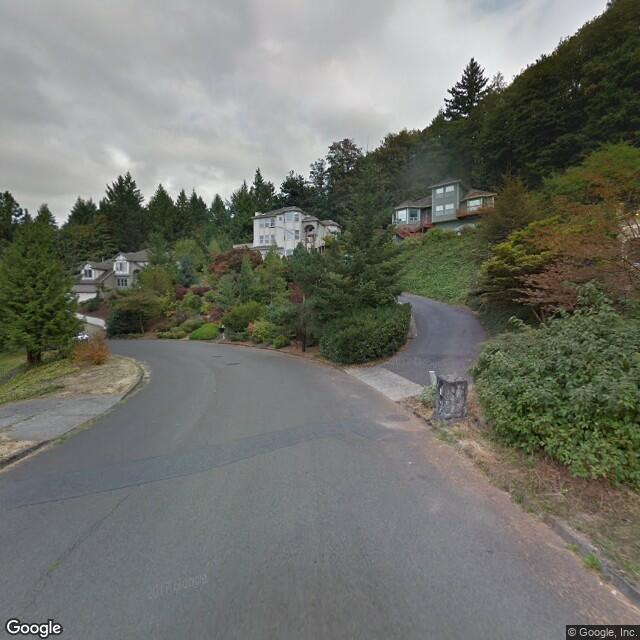
\includegraphics[width=0.25\linewidth]{input.jpg}
	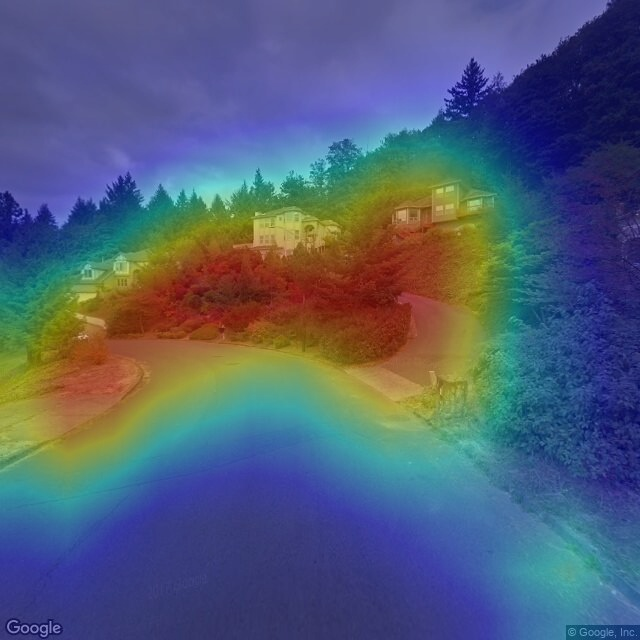
\includegraphics[width=0.25\linewidth]{cam.jpg}
	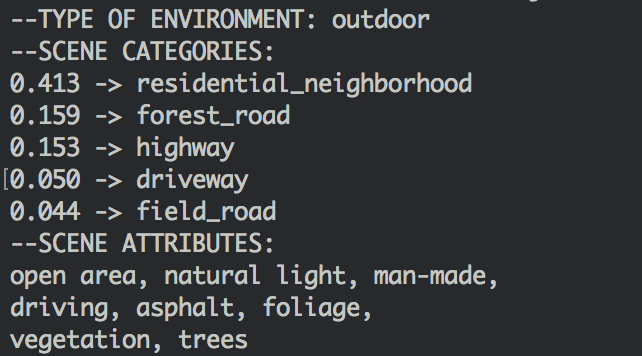
\includegraphics[width=.45\linewidth]{classification.png}
}
   
\end{center}
   \caption{Input image, class activation map, and predicted scene categories and attributes from Places365-ResNet50.}
\label{fig:short}
\end{figure*}

\subsection{Evaluation}

We expect our classifier to be able to classify unseen street-view images as bike-friendly or not with precision and recall better than a naive guess. We plan to train our classifier on a random sample of 80\% of our dataset and evaluate it on the remaining 20\%. Additionally, we expect that the classifier learns sensible low-level features. For example, we expect that images of bike-friendly streets are more likely to contain cyclists in them; they likely contain fewer cars; and they include bike-lane markings. We will consider it a success if our classifier is able to learn to associate these features with bike-designated streets.

%-------------------------------------------------------------------------
\section{Technical Approach}

We will employ transfer learning to adapt an existing convolutional neural network (CNN) to the task of bike-designated road classification. Specifically, we will extend a pre-trained Places365-ResNet50 model. Created by MIT CSAIL, Places365 is a scene classifier based on the Places365 dataset, which contains millions of scene images labeled with 365 semantic categories and additional image attributes. 

Each image the Places365 classifier predicts: 

\begin{itemize}
	\itemsep0em 
	\item scene classification 
	\item attributes
	\item class activation map
\end{itemize}

We will use the ResNet50 implementation of Places365, which achieves the highest top-5 accuracy of all Places365. We will retrain the final layers of the Places365-ResNet50 model, and replace layers to map the classifier to our two predicted classes.

%-------------------------------------------------------------------------
\section{Preliminary Results}

\subsection{Data}

We have generated a labeled dataset of 17,271 Street View images of roads in Boulder, Colorado; Pittsburgh, Pennsylvania; Portland, Oregon; and Seattle, Washington. These cities were selected due to their relative balance between bike-designated roads (55.8\%) versus non-designated roads (44.2\%). Additional data can be added as needed by incorporating new cities or by taking additional Street View images from the same roads (in the reverse direction, or from different points on each road). Manual review of samples of images suggest that the data is very high quality: less than a tenth of a percent of images are misoriented or include artifacts such as the top of the Google Street View car. 

\subsection{Classifier}

We have set up the pre-trained Places365-ResNet50 network in a Google Cloud virtual environment and predicted scene classification and attributes of images in our labeled dataset. The results of the tests are very promising: the classifier is able to identify subtle scene categories and attributes that we expect will be valuable for our binary-classification task.

{\small
\bibliographystyle{ieee}
\bibliography{egbib}
}

\end{document}
